\chapter{Linear Oscillations: Free, Damped, and Forced Resonance}
\label{ch:oscillations}

\begin{chapterintro}
\textbf{Chapter Objectives:} In this chapter, we develop the comprehensive mathematical theory of linear oscillations. You will master the free harmonic oscillator and its phase-space geometry; analyze viscous damping across underdamped, critically damped, and overdamped regimes; quantify energy dissipation via the logarithmic decrement $\delta$ and quality factor $Q$; derive the exact amplitude and phase response of sinusoidally driven oscillators; uncover the distinction between amplitude resonance and velocity resonance; and calculate the normal modes and beat phenomena of coupled oscillators.
\end{chapterintro}

\section{The Free Undamped Harmonic Oscillator}

Any mechanical system possessing a stable equilibrium state obeys, for sufficiently small perturbations, the canonical homogeneous differential equation:
\begin{equation}
\frac{\dd^2 x}{\dd t^2} + \omega_0^2\, x = 0, \qquad \omega_0 \eqdef \sqrt{\frac{k}{m}}.
\end{equation}
The general real solution may be expressed in three equivalent forms:
\begin{align}
x(t) &= A \cos(\omega_0 t + \phi) \\
     &= C_1 \cos(\omega_0 t) + C_2 \sin(\omega_0 t) \\
     &= \operatorname{Re}\left( \underline{X}_0 e^{i\omega_0 t} \right), \quad \underline{X}_0 = A e^{i\phi} \in \mathbb{C}.
\end{align}

\begin{figure}[htbp]
\centering
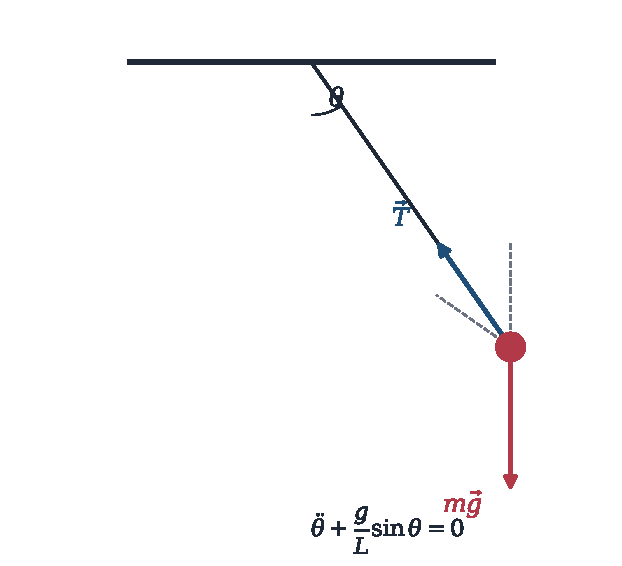
\includegraphics[width=0.72\textwidth]{figures/20_pendulum.pdf}
\caption{The simple gravity pendulum of length $L$. For small angular displacements ($\sin\theta \approx \theta$), the motion is strictly harmonic with angular frequency $\omega_0 = \sqrt{g/L}$. The phase portrait shows concentric elliptical trajectories around the stable center $(0,0)$ and the homoclinic separatrix passing through the unstable inverted equilibrium $(\pm\pi, 0)$.}
\label{fig:pendulum}
\end{figure}

Differentiating with respect to time yields the velocity:
\begin{equation}
v(t) = \dot{x}(t) = -\omega_0 A \sin(\omega_0 t + \phi) = \omega_0 A \cos\left(\omega_0 t + \phi + \frac{\pi}{2}\right).
\end{equation}
\emph{Key kinematic property:} The velocity leads the displacement by a phase quadrature of $\pi/2\ \mathrm{rad}$ ($90^\circ$).

\subsection{Energy and Phase Space Trajectory}

The instantaneous kinetic and potential energies are:
\begin{equation}
E_k(t) = \frac{1}{2}m v(t)^2 = \frac{1}{2}m \omega_0^2 A^2 \sin^2(\omega_0 t + \phi),
\end{equation}
\begin{equation}
E_p(t) = \frac{1}{2}k x(t)^2 = \frac{1}{2}m \omega_0^2 A^2 \cos^2(\omega_0 t + \phi).
\end{equation}
Adding these expressions confirms rigorous energy conservation at every instant:
\begin{equation}
E_m = E_k(t) + E_p(t) = \frac{1}{2}m \omega_0^2 A^2 = \frac{1}{2}k A^2 = \text{constant}.
\end{equation}
Averaging over a full cycle $T_0 = 2\pi/\omega_0$, using $\langle \sin^2 \rangle = \langle \cos^2 \rangle = \frac{1}{2}$:
\begin{equation}
\langle E_k \rangle = \langle E_p \rangle = \frac{1}{4} m \omega_0^2 A^2 = \frac{1}{2} E_m.
\end{equation}
In phase space with coordinates $(x, \dot{x}/\omega_0)$, the trajectory is a circle of radius $A$; in standard phase space $(x, v)$, it is an ellipse of semi-axes $A$ and $\omega_0 A$:
\begin{equation}
\frac{x^2}{A^2} + \frac{v^2}{\omega_0^2 A^2} = 1.
\end{equation}

\begin{historicalbox}{Christiaan Huygens and the Isochronous Pendulum}
\begin{minipage}{0.28\textwidth}
\centering
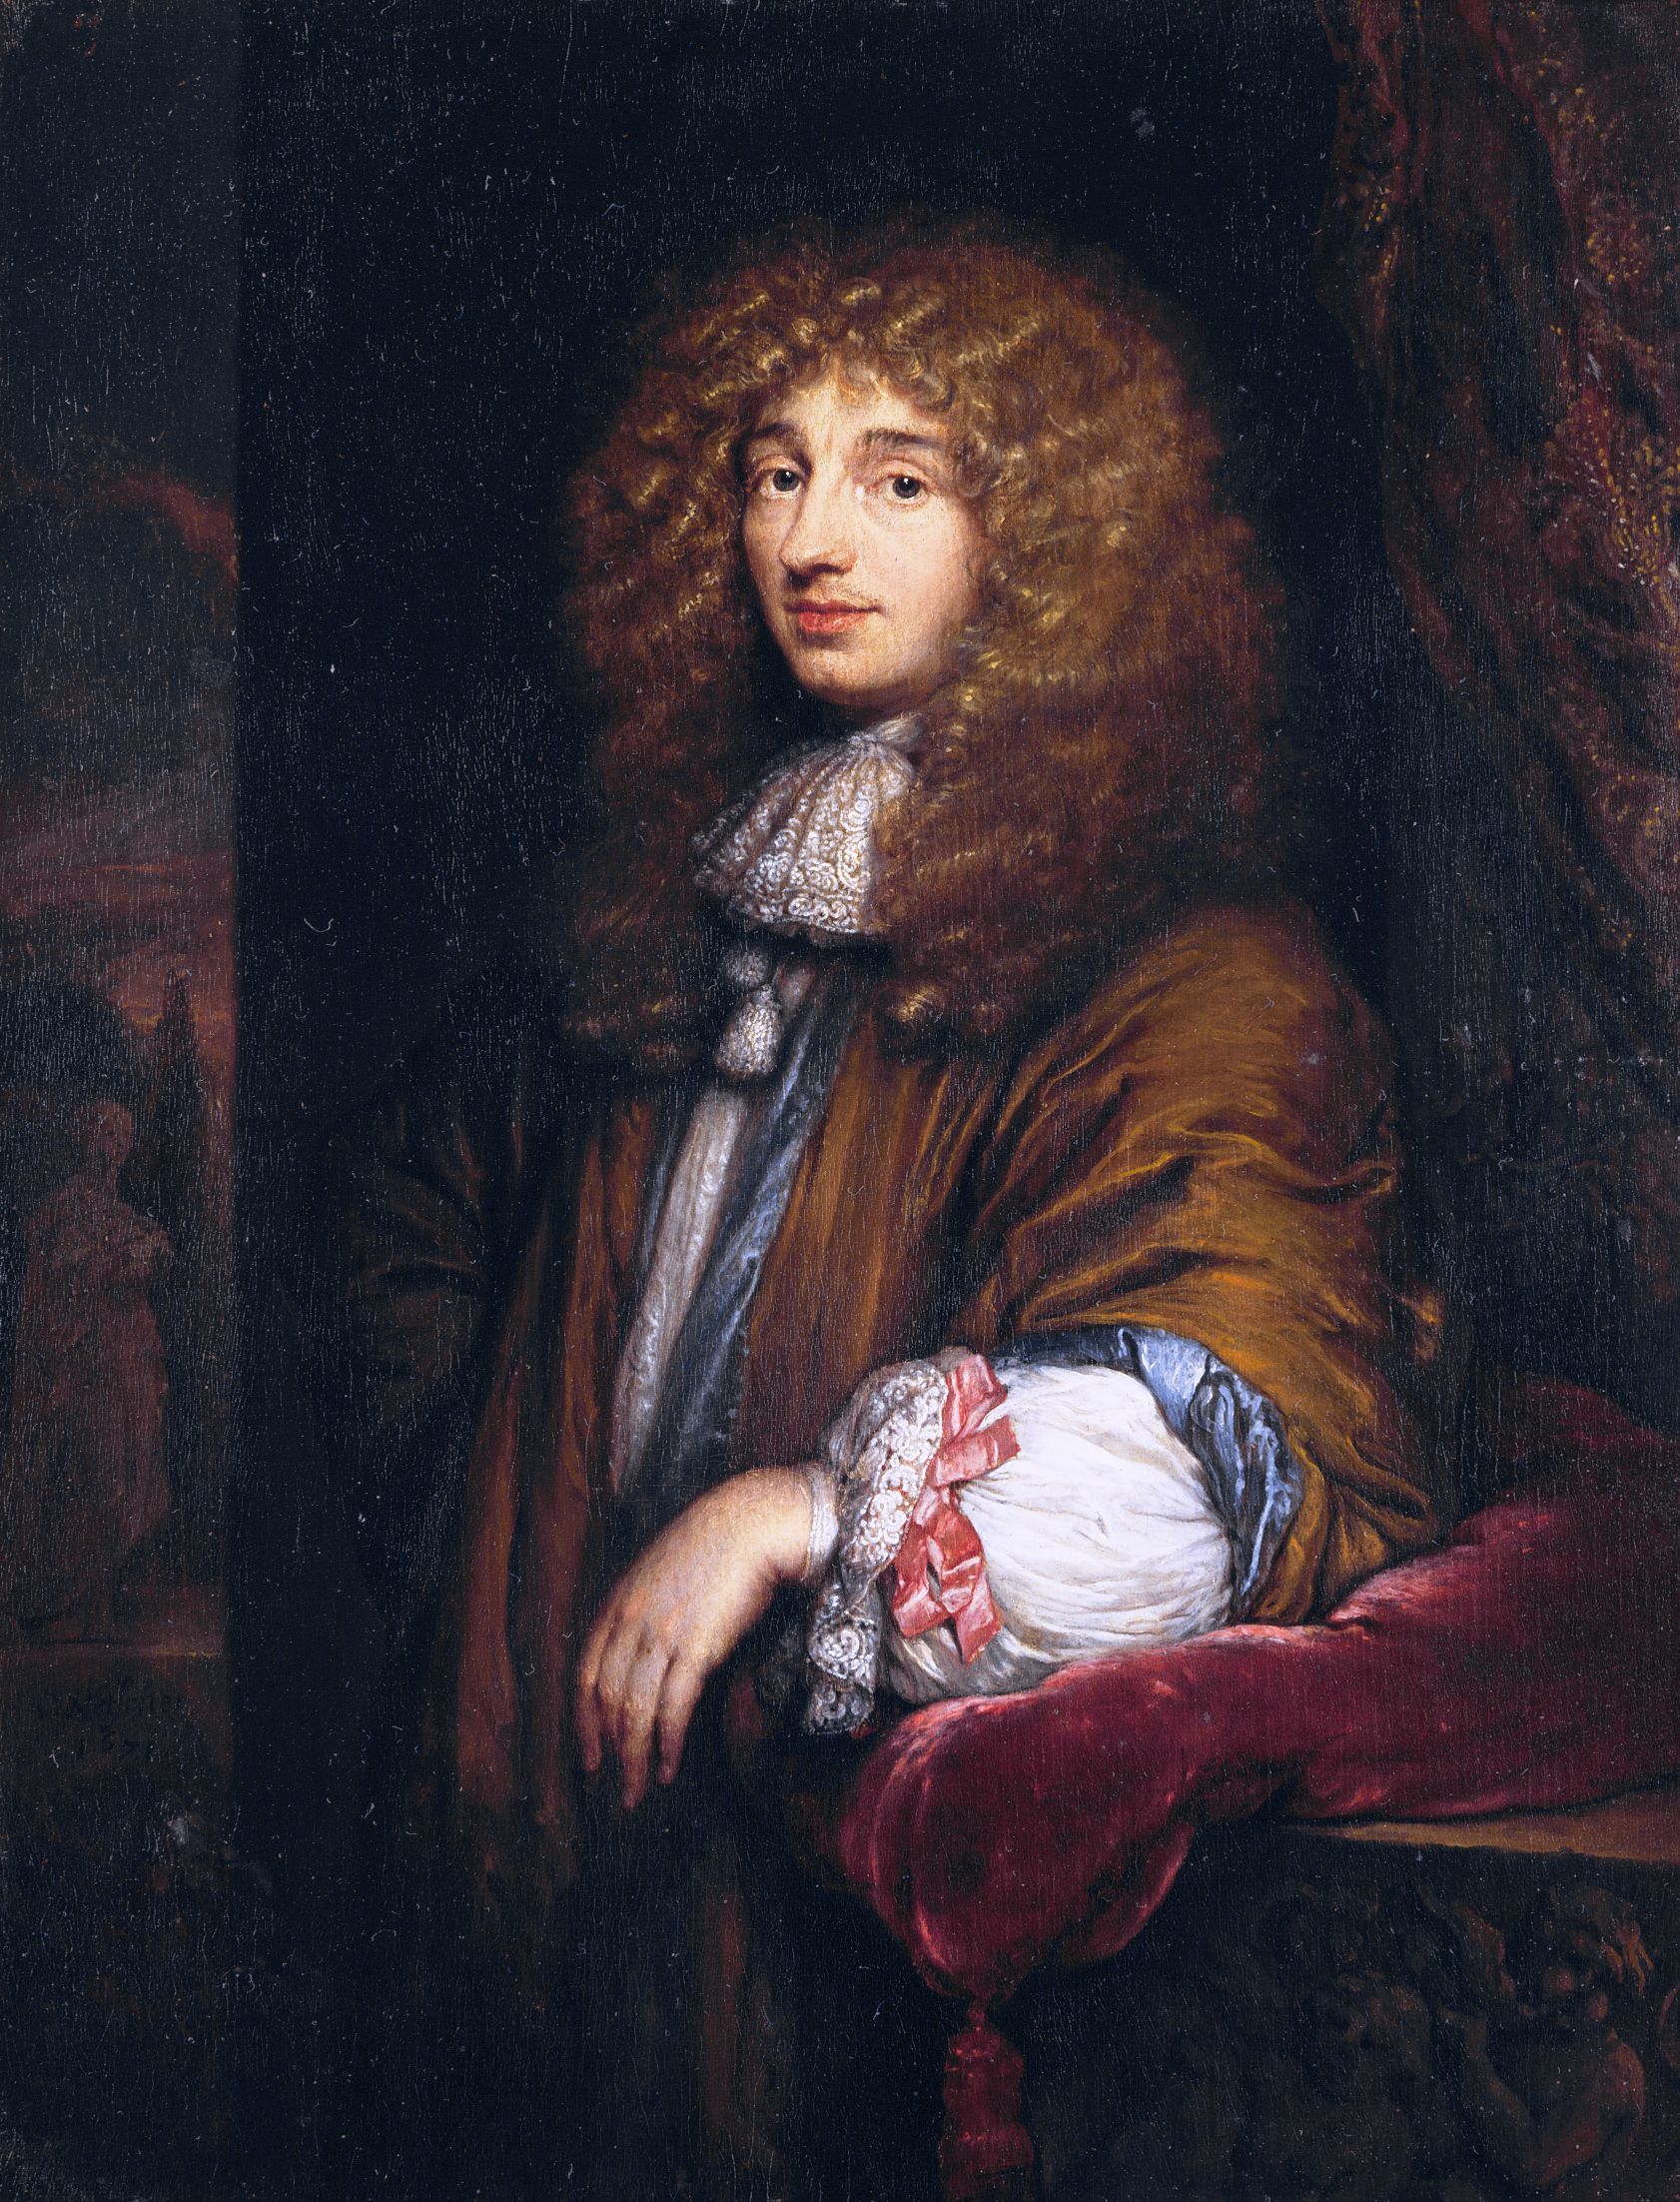
\includegraphics[width=0.92\textwidth]{images/huygens.jpg}
\captionof{figure}{Christiaan Huygens (1629--1695), portrait by Caspar Netscher (1671, Haags Historisch Museum).}
\end{minipage}\hfill
\begin{minipage}{0.68\textwidth}
In 1656, Dutch mathematician and physicist Christiaan Huygens invented the pendulum clock, dramatically increasing timekeeping accuracy from 15 minutes per day to under 15 seconds. In his 1673 masterpiece \emph{Horologium Oscillatorium}, Huygens proved mathematically that while a circular pendulum is only approximately isochronous for tiny angles ($\sin\theta \approx \theta$), a pendulum whose bob is guided between cycloidal cheeks executes \textbf{strictly isochronous oscillations} of period $T = 2\pi\sqrt{L/g}$ regardless of amplitude.

Huygens also made the first recorded observation of \textbf{synchronization} in 1665: two pendulum clocks mounted to the same wooden beam gradually locked into antiphase alignment through minuscule vibrations transmitted through the structure.
\end{minipage}
\end{historicalbox}

\section{Damped Oscillations (Viscous Resistance)}

Real mechanical systems inevitably encounter fluid resistance or internal friction. Modeling the dissipative force as linear viscous damping $\vec{F}_d = -\lambda \vec{v}$ ($\lambda > 0$), Newton's second law reads:
\begin{equation}
m \ddot{x} = -k x - \lambda \dot{x} \implies \ddot{x} + 2\gamma \dot{x} + \omega_0^2 x = 0,
\end{equation}
where we introduce the \textbf{damping parameter} $\gamma$ and the dimensionless \textbf{damping ratio} $\zeta$:
\begin{equation}
\gamma \eqdef \frac{\lambda}{2m}, \qquad \zeta \eqdef \frac{\gamma}{\omega_0} = \frac{\lambda}{2\sqrt{k m}}.
\end{equation}
Seeking solutions of the form $x(t) = e^{r t}$ leads to the characteristic algebraic equation:
\begin{equation}
r^2 + 2\gamma r + \omega_0^2 = 0 \implies r_{1,2} = -\gamma \pm \sqrt{\gamma^2 - \omega_0^2}.
\end{equation}

\begin{figure}[htbp]
\centering
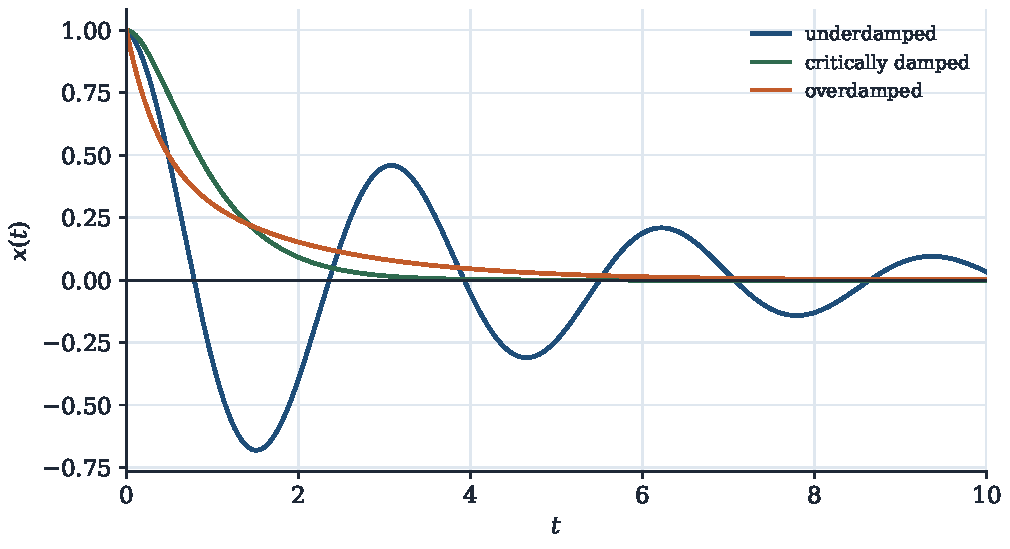
\includegraphics[width=0.74\textwidth]{figures/16_damped_oscillations.pdf}
\caption{Evolution of a damped oscillator for identical initial displacement $x(0) = x_0, \dot{x}(0) = 0$: (1) underdamped oscillatory decay ($\zeta < 1$, blue); (2) critically damped non-oscillatory return ($\zeta = 1$, green); (3) overdamped sluggish relaxation ($\zeta > 1$, red).}
\label{fig:damped_oscillations}
\end{figure}

The nature of the motion depends fundamentally on the sign of the discriminant $\Delta = \gamma^2 - \omega_0^2$:

\subsection{1. Underdamped Regime ($\gamma < \omega_0$, $\zeta < 1$)}
The roots are complex conjugates $r_{1,2} = -\gamma \pm i \omega_d$, where the \textbf{pseudofrequency} is:
\begin{equation}
\omega_d \eqdef \sqrt{\omega_0^2 - \gamma^2} = \omega_0 \sqrt{1 - \zeta^2} < \omega_0.
\end{equation}
The general real solution describes pseudo-periodic oscillations decaying exponentially within an envelope:
\begin{equation}
x(t) = A_0 e^{-\gamma t} \cos(\omega_d t + \phi).
\end{equation}
The \textbf{pseudoperiod} is $T_d = \frac{2\pi}{\omega_d} = \frac{2\pi}{\sqrt{\omega_0^2 - \gamma^2}} > T_0$. Damping systematically lengthens the period of oscillation.

\begin{definitionbox}{Logarithmic Decrement and Quality Factor}
The \textbf{logarithmic decrement} $\delta$ measures the rate of amplitude decay between successive peaks separated by one pseudoperiod $T_d$:
\begin{equation}
\delta \eqdef \ln\left( \frac{x(t)}{x(t + T_d)} \right) = \ln\left( \frac{e^{-\gamma t}}{e^{-\gamma(t + T_d)}} \right) = \gamma T_d = \frac{2\pi \gamma}{\omega_d} = \frac{2\pi \zeta}{\sqrt{1 - \zeta^2}}.
\end{equation}
The dimensionless \textbf{Quality Factor} $Q$ quantifies the sharpness of the oscillator's energy retention:
\begin{equation}
Q \eqdef \frac{\omega_0}{2\gamma} = \frac{1}{2\zeta} = \frac{\sqrt{km}}{\lambda} \approx \frac{\pi}{\delta} \quad (\text{for } Q \gg 1).
\end{equation}
The fractional energy loss per oscillation cycle is related to $Q$ by:
\begin{equation}
\frac{|\Delta E_m|}{E_m} \approx \frac{2\pi}{Q}.
\end{equation}
\end{definitionbox}

\subsection{2. Critically Damped Regime ($\gamma = \omega_0$, $\zeta = 1$)}
The characteristic equation has a degenerate double real root $r = -\gamma$. The general solution is:
\begin{equation}
x(t) = (C_1 + C_2 t) e^{-\gamma t}.
\end{equation}
\emph{Engineering Significance:} Critical damping provides the \textbf{fastest possible return to equilibrium without oscillation or overshoot}. It is the design target for automotive shock absorbers, analog galvanometer meters, and seismic dampers.

\subsection{3. Overdamped Regime ($\gamma > \omega_0$, $\zeta > 1$)}
The roots are distinct, negative real numbers $r_{1,2} = -\gamma \pm \sqrt{\gamma^2 - \omega_0^2} < 0$. The solution is:
\begin{equation}
x(t) = C_1 e^{-(\gamma - \sqrt{\gamma^2 - \omega_0^2})t} + C_2 e^{-(\gamma + \sqrt{\gamma^2 - \omega_0^2})t}.
\end{equation}
The motion is non-oscillatory and exhibits sluggish exponential creeping dominated by the slow decay rate $\lambda_{\text{slow}} = \gamma - \sqrt{\gamma^2 - \omega_0^2}$.

\section{Forced Oscillations and Resonance}

Subjecting the damped oscillator to an external harmonic driving force $F(t) = F_0 \cos(\Omega t)$:
\begin{equation}
\ddot{x} + 2\gamma \dot{x} + \omega_0^2 x = \frac{F_0}{m} \cos(\Omega t).
\end{equation}
The general solution is the superposition of the transient complementary solution $x_h(t)$ (which decays exponentially to zero) and the permanent \textbf{steady-state response} $x_p(t)$:
\begin{equation}
x_p(t) = X_0(\Omega) \cos(\Omega t - \varphi(\Omega)).
\end{equation}

\subsection{Complex Impedance Derivation}
Representing the driving force as $\underline{F}(t) = F_0 e^{i\Omega t}$ and the response as $\underline{x}(t) = \underline{X}_0 e^{i\Omega t}$:
\[
(-\Omega^2 + 2i\gamma\Omega + \omega_0^2) \underline{X}_0 = \frac{F_0}{m} \implies \underline{X}_0 = \frac{F_0 / m}{(\omega_0^2 - \Omega^2) + 2i\gamma\Omega}.
\]
Taking the modulus and argument:

\begin{lawbox}{Resonance Amplitude and Phase Lag}
The steady-state oscillation amplitude is:
\begin{equation}
X_0(\Omega) = \frac{F_0 / m}{\sqrt{(\omega_0^2 - \Omega^2)^2 + 4\gamma^2\Omega^2}} = \frac{F_0 / k}{\sqrt{\left(1 - \frac{\Omega^2}{\omega_0^2}\right)^2 + \frac{1}{Q^2}\left(\frac{\Omega}{\omega_0}\right)^2}}.
\end{equation}
The phase lag $\varphi(\Omega) \in [0, \pi]$ by which displacement trails the force is:
\begin{equation}
\tan\varphi(\Omega) = \frac{2\gamma\Omega}{\omega_0^2 - \Omega^2}.
\end{equation}
\begin{itemize}[leftmargin=1.5em,itemsep=2pt]
  \item At low frequencies ($\Omega \ll \omega_0$): $X_0 \to F_0/k$ (quasi-static response, in phase: $\varphi \to 0$).
  \item At exact tuning ($\Omega = \omega_0$): $\varphi = \pi/2$ (quadrature). The velocity is strictly in phase with the force, maximizing instantaneous power transfer!
  \item At high frequencies ($\Omega \gg \omega_0$): $X_0 \to \frac{F_0}{m\Omega^2} \to 0$ (inertia-dominated, antiphase: $\varphi \to \pi$).
\end{itemize}
\end{lawbox}

\begin{definitionbox}{Amplitude Resonance vs Velocity Resonance}
\begin{itemize}[leftmargin=1.5em,itemsep=3pt]
  \item \textbf{Amplitude Resonance:} The frequency $\Omega_r$ that maximizes $X_0(\Omega)$ minimizes the denominator $f(u) = (\omega_0^2 - u)^2 + 4\gamma^2 u$ (where $u = \Omega^2$):
  \begin{equation}
  \Omega_r = \sqrt{\omega_0^2 - 2\gamma^2} = \omega_0 \sqrt{1 - \frac{1}{2Q^2}}.
  \end{equation}
  Amplitude resonance exists if and only if $\gamma < \omega_0/\sqrt{2}$ ($Q > 1/\sqrt{2} \approx 0.707$).
  At this peak, the maximum amplitude is:
  \begin{equation}
  X_{\max} = X_0(\Omega_r) = \frac{F_0 / m}{2\gamma\sqrt{\omega_0^2 - \gamma^2}} \approx Q \left(\frac{F_0}{k}\right) \quad (\text{for } Q \gg 1).
  \end{equation}
  \item \textbf{Velocity Resonance:} The velocity amplitude $V_0(\Omega) = \Omega X_0(\Omega) = \frac{F_0/m}{\sqrt{(\omega_0^2/\Omega - \Omega)^2 + 4\gamma^2}}$ attains its global maximum \textbf{strictly at $\Omega = \omega_0$} for any level of damping.
  \item \textbf{Half-Power Resonance Bandwidth:} The full width at half-maximum power is:
  \begin{equation}
  \Delta\Omega = 2\gamma = \frac{\omega_0}{Q}.
  \end{equation}
\end{itemize}
\end{definitionbox}

\section{Comprehensive Worked Examples}

\begin{workedexample}{Experimental Determination of Damping and Quality Factor}
A harmonic mass-spring oscillator has inertial mass $m = 0.50\ \mathrm{kg}$ and spring stiffness $k = 200\ \mathrm{N\cdot m^{-1}}$. When set into motion in a viscous liquid, a high-speed camera records that the displacement amplitude decreases by a factor of $3.0$ over $6$ complete oscillation cycles.
\begin{enumerate}[leftmargin=1.4em,itemsep=3pt]
  \item Compute the logarithmic decrement $\delta$ and the damping parameter $\gamma$.
  \item Calculate the viscous damping coefficient $\lambda$ and the Quality Factor $Q$.
  \item Determine the percentage difference between the pseudofrequency $\omega_d$ and the undamped natural frequency $\omega_0$.
\end{enumerate}

\paragraph{Solution.}
\textbf{1. Logarithmic Decrement and Damping Parameter:}\\
The amplitude after $N = 6$ complete periods satisfies:
\[
\frac{A(t)}{A(t + N T_d)} = e^{N \gamma T_d} = 3.0 \implies N \gamma T_d = \ln(3.0) \approx 1.0986.
\]
The logarithmic decrement per single period is:
\[
\delta = \gamma T_d = \frac{\ln(3.0)}{N} = \frac{1.0986}{6} \approx 0.1831.
\]
The undamped angular frequency is:
\[
\omega_0 = \sqrt{\frac{k}{m}} = \sqrt{\frac{200}{0.50}} = \sqrt{400} = 20.0\ \mathrm{rad\cdot s^{-1}}.
\]
Since $\delta = \frac{2\pi \gamma}{\omega_d} = \frac{2\pi \zeta}{\sqrt{1 - \zeta^2}}$, we invert for the damping ratio $\zeta$:
\[
\frac{\zeta^2}{1 - \zeta^2} = \left(\frac{\delta}{2\pi}\right)^2 = \left(\frac{0.1831}{6.2832}\right)^2 = (0.02914)^2 \approx 8.492\times 10^{-4}.
\]
Because $\zeta \ll 1$, to high accuracy $\zeta \approx 0.02914$.
The damping parameter $\gamma$ is:
\[
\gamma = \zeta \omega_0 = (0.02914)(20.0) \approx 0.5828\ \mathrm{s^{-1}}.
\]

\textbf{2. Viscous Coefficient and Quality Factor:}\\
The fluid resistance coefficient $\lambda$ is:
\[
\lambda = 2m\gamma = 2(0.50\ \mathrm{kg})(0.5828\ \mathrm{s^{-1}}) \approx 0.583\ \mathrm{kg\cdot s^{-1}} = 0.583\ \mathrm{N\cdot s\cdot m^{-1}}.
\]
The Quality Factor $Q$ is:
\[
Q = \frac{\omega_0}{2\gamma} = \frac{20.0}{2(0.5828)} = \frac{20.0}{1.1656} \approx 17.16 \approx \frac{\pi}{\delta} = \frac{3.1416}{0.1831} \approx 17.16.
\]

\textbf{3. Frequency Shift:}\\
The pseudofrequency is:
\[
\omega_d = \omega_0\sqrt{1 - \zeta^2} = 20.0\sqrt{1 - (0.02914)^2} = 20.0\sqrt{1 - 0.000849} \approx 20.0(1 - 0.000425) = 19.9915\ \mathrm{rad\cdot s^{-1}}.
\]
The relative frequency shift is:
\[
\frac{\omega_0 - \omega_d}{\omega_0} \approx \frac{1}{2}\zeta^2 = \frac{1}{2}(0.02914)^2 \approx 0.042\% \quad (\text{less than } 1 \text{ part in } 2300!).
\]
Even with substantial amplitude attenuation ($3\times$ reduction in 6 cycles), the frequency of oscillation remains virtually indistinguishable from the undamped resonance.
\end{workedexample}

\begin{workedexample}{Seismic Base Excitation and Vibration Isolation}
A sensitive scientific instrument of mass $m$ is mounted on an elastic suspension of total stiffness $k$ and viscous damper $\lambda$ anchored to a laboratory foundation. During an earthquake, the foundation undergoes horizontal harmonic displacement $y(t) = Y_0 \cos(\Omega t)$.
\begin{enumerate}[leftmargin=1.4em,itemsep=3pt]
  \item Derive the differential equation of motion for the absolute coordinate $x(t)$ of the instrument.
  \item Determine the transmissibility ratio $T_r \eqdef X_0 / Y_0$ of displacement amplitude transmitted to the instrument as a function of the frequency ratio $\beta \eqdef \Omega/\omega_0$ and damping ratio $\zeta$.
  \item Prove that effective vibration isolation ($T_r < 1$) is achieved if and only if $\beta > \sqrt{2}$.
\end{enumerate}

\paragraph{Solution.}
\textbf{1. Differential Equation of Motion:}\\
The spring force depends on relative elongation $\Delta l = x - y$, and the damper force depends on relative velocity $\dot{x} - \dot{y}$:
\[
m \ddot{x} = -k(x - y) - \lambda(\dot{x} - \dot{y}) \implies m\ddot{x} + \lambda\dot{x} + kx = \lambda\dot{y} + ky.
\]
Dividing by $m$ and using $\omega_0^2 = k/m$ and $2\gamma = \lambda/m = 2\zeta\omega_0$:
\[
\ddot{x} + 2\zeta\omega_0 \dot{x} + \omega_0^2 x = 2\zeta\omega_0 \dot{y} + \omega_0^2 y.
\]

\textbf{2. Transmissibility Ratio:}\\
Using complex representation $\underline{y}(t) = Y_0 e^{i\Omega t}$, so $\dot{\underline{y}}(t) = i\Omega Y_0 e^{i\Omega t}$. The driving terms are:
\[
\omega_0^2 \underline{y} + 2\zeta\omega_0 \dot{\underline{y}} = (\omega_0^2 + 2i\zeta\omega_0\Omega) Y_0 e^{i\Omega t}.
\]
Assuming steady-state response $\underline{x}(t) = \underline{X}_0 e^{i\Omega t}$:
\[
\left( -\Omega^2 + 2i\zeta\omega_0\Omega + \omega_0^2 \right) \underline{X}_0 = (\omega_0^2 + 2i\zeta\omega_0\Omega) Y_0.
\]
Dividing by $\omega_0^2$ and introducing $\beta = \Omega/\omega_0$:
\[
\underline{X}_0 = Y_0 \frac{1 + 2i\zeta\beta}{(1 - \beta^2) + 2i\zeta\beta}.
\]
Taking the absolute modulus of the numerator and denominator:
\[
T_r \eqdef \frac{X_0}{Y_0} = \sqrt{\frac{1 + (2\zeta\beta)^2}{(1 - \beta^2)^2 + (2\zeta\beta)^2}}.
\]

\textbf{3. Criterion for Vibration Isolation:}\\
For the suspension to isolate the instrument from floor vibrations, the transmitted amplitude must be strictly smaller than the ground amplitude, $T_r < 1$:
\[
\frac{1 + (2\zeta\beta)^2}{(1 - \beta^2)^2 + (2\zeta\beta)^2} < 1 \iff 1 + (2\zeta\beta)^2 < (1 - \beta^2)^2 + (2\zeta\beta)^2.
\]
Subtracting $(2\zeta\beta)^2$ from both sides:
\[
1 < (1 - \beta^2)^2 \iff (1 - \beta^2)^2 - 1 > 0 \iff \beta^2(\beta^2 - 2) > 0.
\]
Since $\beta > 0$, this inequality is satisfied if and only if:
\[
\beta^2 - 2 > 0 \implies \beta > \sqrt{2} \implies \Omega > \sqrt{2}\,\omega_0.
\]
\emph{Profound Engineering Conclusion:}
\begin{itemize}[leftmargin=1.5em,itemsep=2pt]
  \item For $\Omega < \sqrt{2}\omega_0$, $T_r > 1$: the suspension \textbf{amplifies} foundation vibrations.
  \item At $\Omega = \sqrt{2}\omega_0$, $T_r = 1$ identically, regardless of the value of damping $\zeta$.
  \item To isolate high-frequency equipment or buildings against seismic ground waves, engineers design very ``soft'' suspensions with very low natural frequency $\omega_0$ so that the operating or earthquake frequency satisfies $\Omega \gg \sqrt{2}\omega_0$.
\end{itemize}
\end{workedexample}

\begin{workedexample}{Coupled Oscillators, Normal Modes, and the Phenomenon of Beats}
Two identical carts of mass $m_1 = m_2 = m$ slide along a frictionless horizontal track. Each cart is anchored to an adjacent wall by an outer spring of stiffness $k$, and the two carts are coupled to each other by a central spring of stiffness $k_c$.
\begin{enumerate}[leftmargin=1.4em,itemsep=3pt]
  \item Write Newton's second law for both carts in matrix form $M \ddot{\vec{X}} + K \vec{X} = \vzero$.
  \item Solve the secular eigenvalue equation to find the two normal mode frequencies $\omega_1$ and $\omega_2$ and their corresponding modal eigenvectors.
  \item Cart 1 is initially displaced by $x_1(0) = a$ while cart 2 is held at $x_2(0) = 0$, and both are released from rest. Show that the subsequent motion exhibits beats and compute the beat period $T_{\text{beat}}$.
\end{enumerate}

\paragraph{Solution.}
\textbf{1. Coupled Differential Equations of Motion:}\\
Let $x_1$ and $x_2$ denote the displacements of cart 1 and cart 2 from their respective equilibrium positions.
\begin{align*}
m \ddot{x}_1 &= -k x_1 - k_c (x_1 - x_2) = -(k + k_c) x_1 + k_c x_2, \\
m \ddot{x}_2 &= -k x_2 - k_c (x_2 - x_1) = k_c x_1 - (k + k_c) x_2.
\end{align*}
In matrix notation with $\vec{X} = \begin{pmatrix} x_1 \\ x_2 \end{pmatrix}$:
\[
\begin{pmatrix} m & 0 \\ 0 & m \end{pmatrix} \begin{pmatrix} \ddot{x}_1 \\ \ddot{x}_2 \end{pmatrix} + \begin{pmatrix} k + k_c & -k_c \\ -k_c & k + k_c \end{pmatrix} \begin{pmatrix} x_1 \\ x_2 \end{pmatrix} = \begin{pmatrix} 0 \\ 0 \end{pmatrix}.
\]

\textbf{2. Normal Modes and Eigenvalues:}\\
Seeking harmonic normal mode solutions $\vec{X}(t) = \vec{A} \cos(\omega t)$ leads to the eigenvalue problem:
\[
\det\left( K - \omega^2 M \right) = \det\begin{pmatrix} (k + k_c) - m\omega^2 & -k_c \\ -k_c & (k + k_c) - m\omega^2 \end{pmatrix} = 0.
\]
This yields:
\[
\left[(k + k_c) - m\omega^2\right]^2 - k_c^2 = 0 \implies (k + k_c) - m\omega^2 = \pm k_c.
\]
We obtain two distinct normal mode frequencies:
\begin{itemize}[leftmargin=1.5em,itemsep=3pt]
  \item \textbf{Mode 1 (Symmetric / In-Phase Mode):} Choosing $+k_c$:
  \[
  m\omega_1^2 = (k + k_c) - k_c = k \implies \omega_1 = \sqrt{\frac{k}{m}}.
  \]
  The modal eigenvector satisfies $-k_c A_{11} + k_c A_{12} = 0 \implies A_{11} = A_{12}$.
  \[
  \vec{A}^{(1)} = \frac{1}{\sqrt{2}}\begin{pmatrix} 1 \\ 1 \end{pmatrix}.
  \]
  In this mode, both carts move in perfect synchronization ($x_1(t) = x_2(t)$). The central spring length remains constant ($\Delta l_c = x_1 - x_2 = 0$); it exerts zero force, oscillating at the uncoupled frequency $\sqrt{k/m}$.
  \item \textbf{Mode 2 (Antisymmetric / Out-of-Phase Mode):} Choosing $-k_c$:
  \[
  m\omega_2^2 = (k + k_c) + k_c = k + 2k_c \implies \omega_2 = \sqrt{\frac{k + 2k_c}{m}} > \omega_1.
  \]
  The modal eigenvector satisfies $k_c A_{21} + k_c A_{22} = 0 \implies A_{21} = -A_{22}$.
  \[
  \vec{A}^{(2)} = \frac{1}{\sqrt{2}}\begin{pmatrix} 1 \\ -1 \end{pmatrix}.
  \]
  In this mode, the carts move in exact opposition ($x_1(t) = -x_2(t)$). The central spring is compressed/extended twice as much, providing extra stiffness and raising the frequency.
\end{itemize}

\textbf{3. Superposition and Beat Phenomenon:}\\
The general solution is a linear superposition of the two normal modes:
\[
x_1(t) = C_1 \cos(\omega_1 t + \phi_1) + C_2 \cos(\omega_2 t + \phi_2),
\]
\[
x_2(t) = C_1 \cos(\omega_1 t + \phi_1) - C_2 \cos(\omega_2 t + \phi_2).
\]
Applying initial conditions: $x_1(0) = a, x_2(0) = 0, \dot{x}_1(0) = 0, \dot{x}_2(0) = 0$:
\[
C_1 + C_2 = a, \qquad C_1 - C_2 = 0 \implies C_1 = C_2 = \frac{a}{2}, \quad \phi_1 = \phi_2 = 0.
\]
The exact trajectories of the two carts are:
\begin{align*}
x_1(t) &= \frac{a}{2}\left( \cos(\omega_1 t) + \cos(\omega_2 t) \right) = a \cos\left(\frac{\omega_2 - \omega_1}{2} t\right) \cos\left(\frac{\omega_2 + \omega_1}{2} t\right), \\
x_2(t) &= \frac{a}{2}\left( \cos(\omega_1 t) - \cos(\omega_2 t) \right) = a \sin\left(\frac{\omega_2 - \omega_1}{2} t\right) \sin\left(\frac{\omega_2 + \omega_1}{2} t\right).
\end{align*}
For weak coupling ($k_c \ll k$), $\omega_2 \approx \omega_1$, defining the mean carrier frequency $\bar{\omega} = \frac{\omega_1 + \omega_2}{2}$ and the modulation frequency $\omega_{\text{mod}} = \frac{\omega_2 - \omega_1}{2} \ll \bar{\omega}$.

The energy sloshes periodically back and forth between cart 1 and cart 2. When cart 1 is at maximum amplitude, cart 2 is momentarily stationary, and vice versa.
The beat period (time between successive amplitude nulls for cart 1) is:
\[
T_{\text{beat}} = \frac{2\pi}{\omega_2 - \omega_1} \approx \frac{2\pi}{\sqrt{\frac{k+2k_c}{m}} - \sqrt{\frac{k}{m}}} \approx \frac{2\pi}{\sqrt{\frac{k}{m}}\left(1 + \frac{k_c}{k} - 1\right)} = \frac{2\pi}{\omega_0} \frac{k}{k_c}.
\]
\end{workedexample}
